\chapter{General discussion}\label{ch:5}

The previous chapter presented the main intonational patterns in L2 Spanish and L2 Italian by offering a multidirectional cross-linguistic comparison that allowed us to examine L1-dependent features and to discern whether there were features common to all learners, independently of their L1 or any particular target language. The overall findings suggest that the cross-linguistic influence strongly determines the interlanguage intonation across all varieties and sentence types. However, we also saw that CLI does not account for all the patterns observed.


The objective of this chapter is to summarize the most important findings and discuss the following issues: In \sectref{sec:5.1} we will examine the areas in which interlanguage varieties differ from one another. In \sectref{sec:5.2} we will reflect on how accurately the learners performed when compared with L1 speakers and speculate about how L2 intonation can be improved. We will then address the question as to whether intonation deviations are equally reflected in the four dimensions of intonation assumed in the LILt in \sectref{sec:5.3}. And, finally, in \sectref{sec:5.4} we will see what the findings tell us about possible developmental sequences in terms of L2 intonation learning.


\section{Interlanguage varieties in contrast}\label{sec:5.1}  %5.1 /

\textit{In which areas do interlanguage varieties differ from one another? Do Spanish interlanguages with L1 Czech and L1 German show larger differences than the two interlanguages with L1 Czech only?}


The previous chapter reported results and offered descriptive statistics for each tonal event and each type of sentence. Next to the occurrences of all tonal events in L2 Spanish and L2 Italian, the mean percentage difference was computed in order to compare how the learner varieties differed from each other. The aim of the summary presented below (Figures~\ref{fig:5.1a}--\ref{fig:5.1e}) is to offer a quick overview of these average differences we presented in the previous chapter. On the whole, L1 Czech learners of Spanish differ more from L1 Czech learners of Italian (18.8\%) than L1 Czech learners of Spanish differ from L1 German learners of this language (16.7\%). This supports the idea that the learners \textit{notice} (in the sense of \citealt{Schmidt1990}, \sectref{sec:2.1.5}) and thus produce the target Romance languages differently. All the Spanish and Italian interlanguages seen here present intonation deviations or innovations (see also \sectref{sec:5.3}). Their strength may be due to various factors; the present study focused on L1 background (\sectref{sec:5.2}) and language proficiency (\sectref{sec:5.4}). Before we examine the accuracy and intonational patterns in the learners’ productions in \sectref{sec:5.2}, let us take a closer look at the differences across the interlanguage varieties according to sentence type and tonal event.

As regards neutral statements (\figref{fig:5.1a}), we find the following picture: the learner varieties differ largely in the realization of pitch accents (especially in medial positions), whereas they show minimal differences in the realization of boundary tones. This is mostly related to cross-linguistic dissimilarities or similarities. For example, due to L1-to-L2 transfer, German learners realized L+H* in nuclear position quite often, whereas Czech learners did not. German learners also exhibited more difficulties with the realization of the prenuclear patterns. In this sentence type, there are more differences between German and Czech learners of Spanish than between Czech learners of Spanish and Czech learners of Italian. This tendency changes with other sentence types, but why this happens remains somewhat puzzling. It could be that neutral statements are not prosodically as salient as other types of sentence and the learners tend to realize them with L1-based patterns more frequently.

\begin{figure}
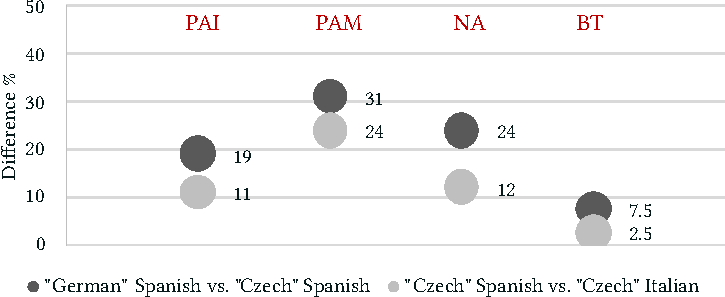
\includegraphics[width=\textwidth]{figures/a05HabilDiscussion-img001.pdf}
\caption{The mean differences between interlanguages in neutral statements\label{fig:5.1a}}
\end{figure}

Biased statements (\figref{fig:5.1b}) exhibit the largest differences again in prenuclear positions. Moreover, we find a larger gap in the realization of nuclear accents: whereas German and Czech learners are quite similar and differ by only 10\%, the two groups of Czech learners differ from each other by 28\%. This is due to the fact that Italian learners acquired quite successfully the target (L+)H*+L pitch accent, a pattern, which does not exist in L1 German, Czech or Spanish. It should be remembered that (L+)H*+L appears only in nuclear position in L1 Italian; however, the L2 Italian data display this pattern (albeit sporadically) in prenuclear positions too. I interpret this “error” as an acquisition strategy and classify it as a case of prosodic overgeneralization that results from an inappropriate application of tonal rules (see \sectref{sec:5.3}). And finally, the smallest difference is found with boundary tones. However, it should be added that German and Czech learners of Spanish completely failed to produce the target L!H\% pattern for expressing obviousness (see \sectref{sec:5.2}).

\begin{figure}
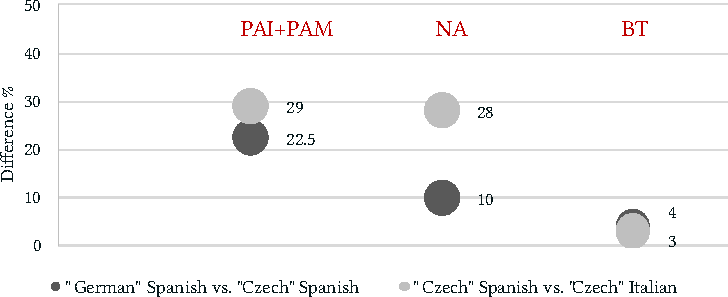
\includegraphics[width=\textwidth]{figures/a05HabilDiscussion-img002.pdf}
\caption{The mean differences between interlanguages in biased statements\label{fig:5.1b}}
\end{figure}

Yes/no questions (\figref{fig:5.1c}) reveal the lowest average differences between the learner varieties, in comparison to the rest of the sentence types. All the learners of Spanish were quite successful in the acquisition of yes/no questions, mainly in producing the rising terminals. Nevertheless, L2 yes/no questions -- and especially biased questions -- still exhibit many transferred features. Moreover, any interpretation of the average differences should be undergone with caution. For example, Czech learners differ from German learners of Spanish by only 8.6\% for all detected boundary tones (H\%, L\%, (H)!H\%, HL\%, LH\%). But a close examination of the results (\sectref{sec:4.3.2}, \tabref{tab:4.18}) shows that the learners differ from each other by 17\% in terms of the use of L\% and H\%, a result that was statistically significant.

\begin{figure}
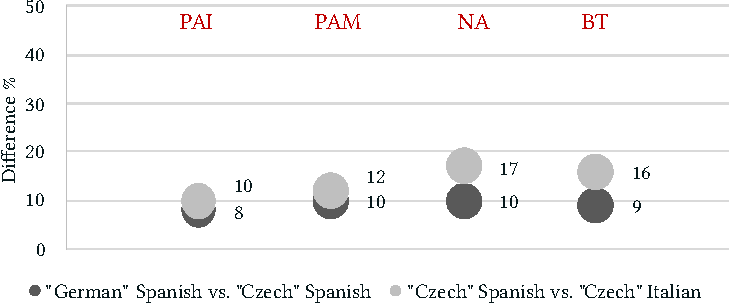
\includegraphics[width=\textwidth]{figures/a05HabilDiscussion-img003.pdf}
\caption{The mean differences between interlanguages in yes-no questions\label{fig:5.1c}}
\end{figure}

Regarding all wh-questions (\figref{fig:5.1d}), much larger differences are again present, mainly in nuclear positions and boundary tones. This is mostly due to the realization of biased wh-questions, where L1 transfer is relatively strong and differences between languages were relatively big. And finally, L2 vocatives show an unexpected result (\figref{fig:5.1e}). In contrast to other sentence types, where L1-to-L2 transfer was predictable, the vocatives revealed the largest difference between the learner varieties. The performance of L2 Italian learners, specifically their overuse of H*+L pitch accents, which I proposed to interpret as a case of prosodic (over)generalization, was discussed at length in \sectref{sec:4.5.5}.

\begin{figure}
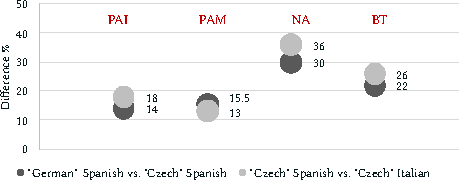
\includegraphics[width=\textwidth]{figures/a05HabilDiscussion-img004.pdf}
\caption{The mean differences between interlanguages in wh-questions\label{fig:5.1d}}
\end{figure}

In concluding this section, it should be emphasized that the summary does not include differences in pitch changes or duration, where further divergences were observed. Nor do the differences presented here reflect \textit{accuracy} either. This issue will be dealt with in the section that follows.

\begin{figure}
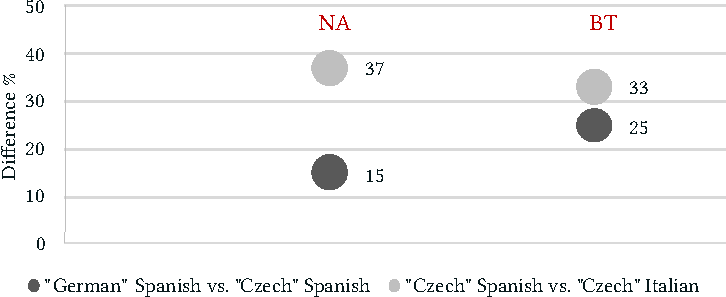
\includegraphics[width=\textwidth]{figures/a05HabilDiscussion-img005.pdf}
\caption{The mean differences between interlanguages in vocatives\label{fig:5.1e}}
\end{figure}

\section{Accuracy in L2 and the role of L1}\label{sec:5.2} %5.2 /

As noted, the summary provided in the previous section says nothing about how accurately L2 learners performed when compared with L1 speakers. The aim of this section is to summarize and discuss the results with regard to accuracy, in a sense how far the learners resembled L1 speakers of the target language. Accuracy refers here to the \textit{appropriate} choice of the phonological pattern to express a specific meaning. In comparison to syntactic, morphological and also segmental phenomena, intonational deviations from the target patterns are much more difficult to pin down; in other words, it is challenging to decide what is actually “accurate” or “correct” and what is “wrong”. Before I propose a model, it is worth noting some of the reasons why it can be difficult to define accuracy. They include:

\begin{itemize}
\item A \textit{high degree of inter-speaker variation} in the L1, which can have diatopic, diaphasic, diastratic but also idiolectal explanations. For example, Spanish speakers 1 and 5 differed systematically in their production of nuclear configurations of yes/no questions, even though they both came from Ciudad Real and were the same age. This is the first factor that makes it complicated to establish a “native norm” that can serve as a reference point for non-native accuracy. It should also be added that there are only a few sociolinguistic studies on intonation (see, e.g., \citealt{EnbeTobin2008}), and thus we are not aware of the extent of the variation in a given population. As already pointed out in \chapref{ch:3}, \textit{\nameref{ch:3}}, the control participants in the present study sometimes diverged from the patterns described in the literature. For example, they did not always realize the expected L+<H* in the prenuclear position of declaratives. Nevertheless, the controls were quite consistent in their productions, meaning that the intra-speaker variation was low.

\item \textit{Limited L1 data in previous research}. It was not always clear which patterns were “accurate” in the prenuclear parts and especially the realization of medial positions in different types of utterances. This is because previous research on L1 has mainly focused on the very first pitch accent or the nuclear configurations -- positions that are usually considered more relevant for meaning (see, e.g., \citealt{Ladd2008}). Another related issue is the mutual influence of tones. In several cases I observed that the realization of one tonal event could be affected by the realization of the preceding one, or the realization of one pitch accent type could influence the subsequent tonal event. Furthermore, data examined in previous research has mostly been limited to short sentences. The present study showed that, for example, longer wh-questions might have different nuclear configurations than shorter ones. A short wh-question in Spanish like \textit{¿Qué hora es?} typically terminates with L* L\%, whereas a longer wh-question like \textit{¿Dónde está la iglesia de San Antonio?} ends with L+H* L\%. The latter configuration is assumed to be characteristic of narrow focus statements, exclamative statements or echo yes/no questions but not of wh-questions in Spanish (see \citealt{Estebas-VilaplanaPrieto2010}). Furthermore, an initial pitch accent in wh-questions can also have a different realization depending on the length of the wh-word and the length of the whole sentence.

\item The \textit{complexity of the prosodic structure}. Intonation interacts simultaneously with further prosodic phenomena and also with gestures and the use of lexical elements that can all convey meaning. The greatest challenge for intonationists is to understand and separate linguistic from paralinguistic meaning (see, e.g., \citealt{Ladd2008, Arvaniti2022}). Our full understanding of this interplay in L2 (and L1) is still limited.
\end{itemize}

In spite of the difficulties outlined above, I will make a preliminary proposal for how the production accuracy of L2 intonation patterns can be measured. This involves creating an “ideal” L1 speaker with typical intonation patterns that can serve as a reference for measuring and comparing accuracy across interlanguage varieties. It should be pointed out expressly and most emphatically that the “ideal speaker’s intonation” is not to be understood as a norm but rather as a preliminary and orientative tool helpful for comparing interlanguages as well as L1 and L2 in order to test hypotheses and predict difficulties learners might have in the target language. The defining of a “prototypical” speaker of Spanish or Italian could also serve didactical purposes to improve non-native intonation.


In order to start somewhere, I defined an “ideal” speaker according to the most typical patterns reported in the literature (\citealt{HualdePrieto2015} for Spanish; \citealt{GiliFivelaEtAl2015} for Italian) and to the data provided by the control participants in the present study. I decided to base the model on Spanish intonation on Peninsular (Madrid) Spanish, simply because the Czech and German learners selected for the present study had had more experience with the variety of Spanish spoken in Europe. As for the Italian “ideal” speaker, I attempted to form a kind of “pan-Italian” typical model, in which the most frequent cross-dialectal patterns would be present. The pan-Italian model seems to be appropriate and possible for broad-focus sentences, vocatives (initial calls) and wh-questions and in phonetic terms also for contrastive-corrective focus. On the contrary, the pan-Italian pattern for yes/no questions, where a large variety of L1 tones is known, is very difficult if not impossible (see, e.g., \citealt{GiliFivelaEtAl2015} for an overview).\footnote{I am grateful for the comment on this issue to one of the two anonymous reviewers of the manuscript.} Yes/no questions exhibit a large degree of variation in Spanish too. To provide a provisional solution here, the accuracy model is based on the controls selected for this study that pertain to the varieties spoken also by (most of) the learners.



It must be added that the accuracy model I propose here does not include any phonetic detail with regard to pitch range, pitch slope, duration or any other parameters that can also play a role. Furthermore, the present study leaves several questions unanswered, particularly with regard to how accuracy in L2 intonation is related to the accentedness (see \citealt{Piske2008}) and how L2 intonation is perceived by natives. Two methods for studying the contribution of intonation to the perception of foreign accent would be deemed to be useful here, namely low-pass filtering that eliminates most segmental information (see, e.g., \citealt{Jilka2000}) and close copy and standardized stylizations of F0 contours (see, e.g., \citealt{Collier1989}); this latter technique allows the researcher to determine which changes in F0 are relevant for the perception of speech melody. Simple identification tests based on native listeners with zero knowledge of the learners’ L1 (see, e.g.,  \citealt{CortésMoreno1998}) could provide an alternative solution for defining accuracy in L2 intonation and explaining the role of L2 intonation in the perception of foreign accent in general.



In the following section, I will summarize the results for accuracy of the interlanguages in overall terms, setting aside the issue of individual accuracy.


\subsection{Accuracy according to sentence type and tonal event}\label{sec:5.2.1}

The findings suggest that both deviations from and agreements with target tonal patterns are more closely linked to the learners’ L1s. Very broadly speaking we can conclude that if the languages profit from positive transfer, the accuracy is high. In the case of negative transfer, the accuracy decreases. Of course, the learners also show (non-)accuracy in patterns that do not originate from positive or negative transfer only (for details see \chapref{ch:4}).


I will now examine the group accuracy in neutral statements, which comprised the sentences \textit{I prefer tangerines} and \textit{Marisa eats tangerines}. \figref{fig:5.2} illustrates the idealized contours for Italian and Spanish and \figref{fig:5.3} the results for accuracy broken down by tonal event and learner variety. With the exception of the boundary tones, Czech learners performed better than German learners. The “Czech” Spanish interlanguage showed better scores in the initial position than the “Czech” Italian interlanguage. This is because L1 Spanish and L1 Czech are phonetically more similar here. Based on CLI, all three interlanguage varieties show a very high accuracy for boundary tones; the lowest accuracy is shown for prenuclear pitch accents (BT > NA > PAI > PAM).

\vfill
\begin{figure}[H]
%%\includegraphics[width=\textwidth]{figures/a05HabilDiscussion-img006.emf}
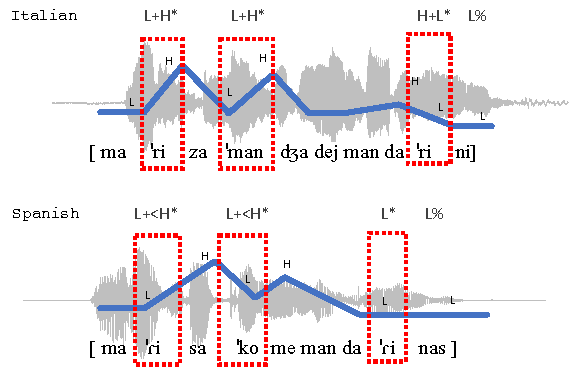
\includegraphics[width=.9\textwidth]{figures/fig52.pdf}
\caption{Idealized contours of neutral (SVO) statements in L1 Italian and L1 Spanish.}
\label{fig:5.2}
\end{figure}
\vfill\pagebreak

\begin{figure}

%%\includegraphics[width=\textwidth]{figures/a05HabilDiscussion-img007.emf}
\begin{tikzpicture}
\tikzset{every node/.style={font=\small}}
\begin{axis}[
  ybar=4pt,
  axis lines*=left,
  width = \textwidth,
  height=.3\textheight,
  ymin = 0,
  ymax = 100,
  ylabel = Accuracy \%,
  xtick = {1,2,3,4},
  xticklabels = {PAI,
  PAM,
  NA,
  BT,
  },
%  enlarge x limits = .06,
  bar width = 10,
  x tick label style = {font=\small},
  nodes near coords,
  legend pos = north west,
]
\addplot+[color = black, opacity = .2]
coordinates{
(1,17.5)
(2,0)
(3,20)
(4,100)
};
\addplot+[color = black, opacity = .5]
coordinates{
(1,45)
(2,10)
(3,50)
(4,92.5)
};
\addplot+[color = black, opacity = 1]
coordinates{
(1,25)
(2,25)
(3,52.5)
(4,95)
};
\legend{``German'' Spanish,``Czech'' Spanish,``Czech'' Italian}
\end{axis}
\end{tikzpicture}




\caption{Accuracy in neutral statements broken down by tonal event and learner variety. ``Ideal L1 speaker'': Spanish: L+<H* (L+<H*) L* L\%; Italian: L+H* (L+H*) H+L* L\%.}
\label{fig:5.3}
\end{figure}

In accordance with the LILt, the accuracy depends on contrasts between L1 and L2 and the position of the tonal event in an utterance. Due to positive transfer, it is not surprising that learners reproduced the boundary tones of statements most accurately. But the tendency observed in statements leads us also into a discussion of whether the boundary tones are acquired first because they are more prominent and together with nuclear accents the main bearers of meaning (see, e.g., \citealt{Ladd2008}). In contrast, the prenuclear positions are considered less prominent and tonal variation observed in these positions might be due to their lesser impact on meaning (see, e.g., \citealt{GrabeEtAl2005}). Medial positions showed the worst score. Interestingly, this fits with the psycholinguistic observation that people notice and remember more beginnings and ends of words than their middle (a phenomenon called the \textit{bathtub effect}). This explanation is quite convincing for statements. However, if we look at the accuracy in other types of sentences (e.g., wh-questions, vocatives), we see that the L1, and not the position in the utterance, seems to be still the most relevant factor in the realization of the respective tonal events (see below). Of course, we cannot exclude the possibility that acquisition and processing of statements is not the same as the acquisition and processing of questions.


With respect to narrow contrastive focus statements (\textit{No, oranges!}), German learners performed slightly better than Czech learners in L2 Spanish due to positive transfer (BT > NA) (Figures~\ref{fig:5.4}, \ref{fig:5.5}). In L2 Italian, Czech learners exhibited less accuracy for the nuclear accents. This is not surprising, because the tonal configuration (L+)H*+L represented a new category for them to learn. It should be added that the learners of Italian also produced the nuclear accents with H+L* quite often (in just two cases, the nuclear accent was realized with L+H*). We could interpret H+L* as a phonetic variant of (L+)H*+L and approximation to the target pattern. This would mean that accuracy is much higher and that the learners struggle with the phonetic implementation of the target tonal patterns.

\vfill
\begin{figure}[H]
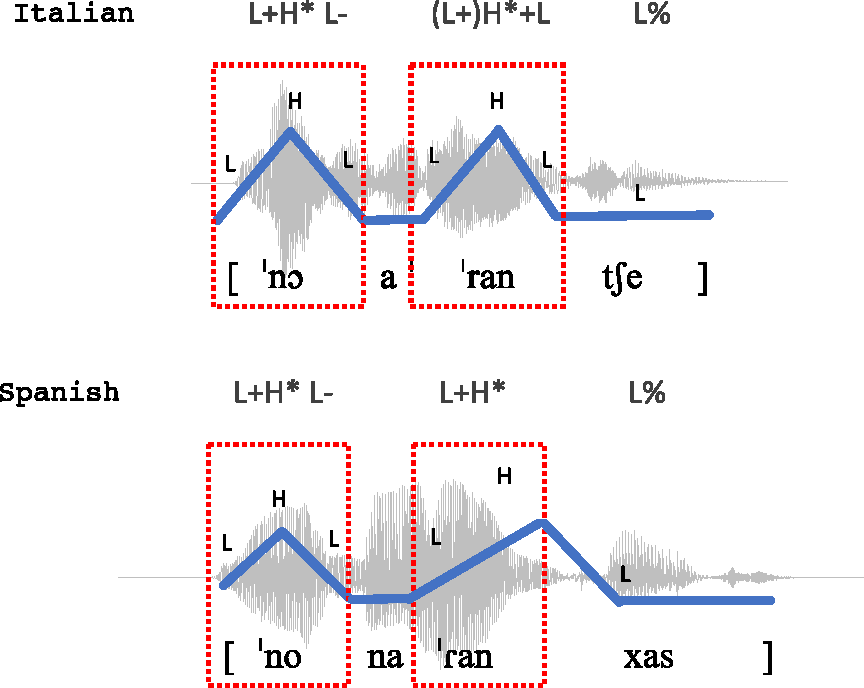
\includegraphics[width=.7\textwidth]{figures/a05HabilDiscussion-img008.pdf}
\caption{Idealized contours of contrastive narrow focus statements in L1 Italian and L1 Spanish.}
\label{fig:5.4}
\end{figure}
\vfill
\begin{figure}[H]
\begin{tikzpicture}
\tikzset{every node/.style={font=\small}}
\begin{axis}[
  ybar=4pt,
  axis lines*=left,
  width = .6\textwidth,
  height=.3\textheight,
  ymin = 0,
  ymax = 100,
  ylabel = Accuracy \%,
  xtick = {1,2,3,4},
  xticklabels = {
  NA,
  BT,
  },
  enlarge x limits = .5,
  bar width = 10,
  x tick label style = {font=\small},
  nodes near coords,
  legend pos = outer north east,
]
\addplot+[color = black, opacity = .2]
coordinates{
(1,90)
(2,100)
};
\addplot+[color = black, opacity = .5]
coordinates{
(1,80)
(2,90)
};
\addplot+[color = black, opacity = 1]
coordinates{
(1,60)
(2,95)
};
\legend{``German'' Spanish,``Czech'' Spanish,``Czech'' Italian}
\end{axis}
\end{tikzpicture}
\caption{Accuracy in narrow focus statements broken down by tonal event and learner variety. ``Ideal L1 speaker'': Spanish: L+H* L\%; Italian: (L+)H*+L L\%.}
\label{fig:5.5}
\end{figure}
\vfill\pagebreak


With regard to another type of biased statement expressing the obvious (\textit{With Manuel (obviously)! It is John Travolta (obviously)!}), accuracy is high and similar to the preceding marked structures in L2 Italian (BT > NA). Both Czech and German learners of Spanish failed to realize the L!H\% boundary tone: either the learners had not received enough access to this type of structure (input limitation) or they associate the high tone merely with questions (semantic limitation), or both together. Due to the variability also found in L1 Spanish controls, a question that requires an answer is whether natives would interpret statements of the obvious as such also with other tones than L!H\% (for more details on non-neutral statements in L2 Italian and L2 Spanish see \citealt{Pešková2022b}).


\begin{figure}

%%\includegraphics[width=\textwidth]{figures/a05HabilDiscussion-img010.emf}
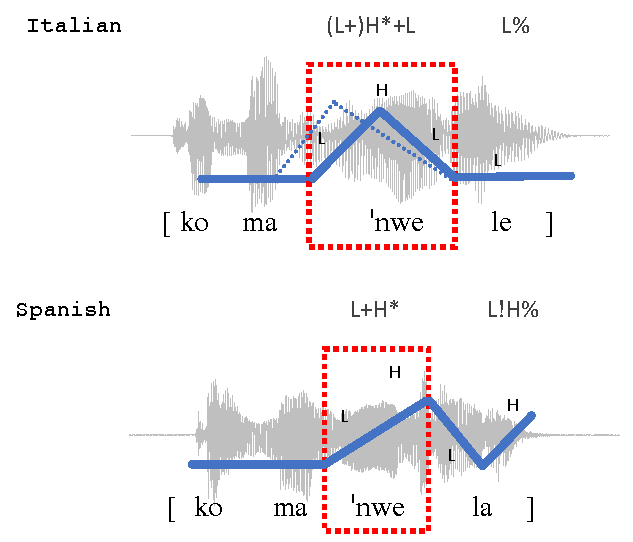
\includegraphics[width=.7\textwidth]{figures/fig56.pdf}
\caption{Idealized contours of statements of the obvious in L1 Italian and L1 Spanish. The dotted line represents another common pitch movement. I use the name \textit{Manuela} (paroxytone word) here instead of \textit{Manuel} (oxytone word) to better illustrate the pitch track.}
\label{fig:5.6}
\end{figure}

\begin{figure}

%%\includegraphics[width=\textwidth]{figures/a05HabilDiscussion-img011.emf}
\begin{tikzpicture}
\tikzset{every node/.style={font=\small}}
\begin{axis}[
  ybar=4pt,
  axis lines*=left,
  width = .6\textwidth,
  height=.3\textheight,
  ymin = 0,
  ymax = 100,
  ylabel = Accuracy \%,
  xtick = {1,2,3,4},
  xticklabels = {
  NA,
  BT,
  },
  enlarge x limits = .5,
  bar width = 10,
  x tick label style = {font=\small},
  nodes near coords,
  legend pos = outer north east,
]
\addplot+[color = black, opacity = .2]
coordinates{
(1,100)
(2,5)
};
\addplot+[color = black, opacity = .5]
coordinates{
(1,85)
(2,2.5)
};
\addplot+[color = black, opacity = 1]
coordinates{
(1,62.5)
(2,93)
};
\legend{``German'' Spanish,``Czech'' Spanish,``Czech'' Italian}
\end{axis}
\end{tikzpicture}



\caption{Accuracy in statements of the obvious broken down by tonal event and learner variety. ``Ideal L1 speaker'': Spanish: L+H* L!H; Italian: (L+)H*+L L\%.}
\label{fig:5.7}
\end{figure}


Now we turn our attention to neutral yes/no questions (Figures~\ref{fig:5.8}, \ref{fig:5.9}) and neutral wh-questions (Figures~\ref{fig:5.10}, \ref{fig:5.11}). Biased yes/no questions and biased wh-questions are left out of a discussion because of the wide range of pragmatic nuances and variation they involve. In neutral yes/no questions (\textit{Do you have tangerines? May I sit down? Shall we go for a beer?}), the results show a very mixed picture. First, German learners of Spanish performed much better, benefiting from positive transfer. They show more accurate patterns in the nuclear position and boundary tones than in initial or medial positions (BT > NA > PAI > PAM). We also saw a better accuracy in pitch change. Czech learners of Spanish show a similar tendency but with lower accuracy rates and differences in the prenuclear position (BT > NA > PAM > PAI). Due to positive transfer, Czech learners of Italian produce the medial positions very accurately, followed by nuclear and initial positions (PAM > NA > PAI > BT). The low accuracy of the target boundary tones (LH\%) in Italian interlanguage might be due to the problems in the phonetic dimension since the learners used a high tone with different shapes: H\% (without an apparent L target), H!H\% or !H\%. Such patterns were observed in their L1 Czech.


\begin{figure}

%%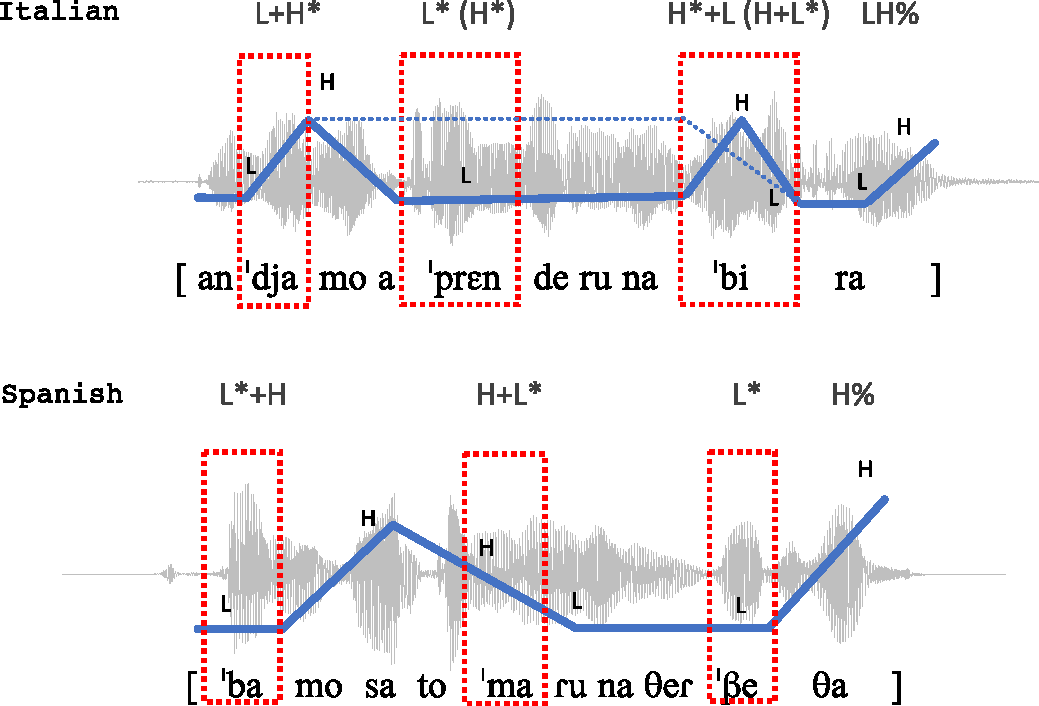
\includegraphics[width=\textwidth]{figures/a05HabilDiscussion-img012.emf}
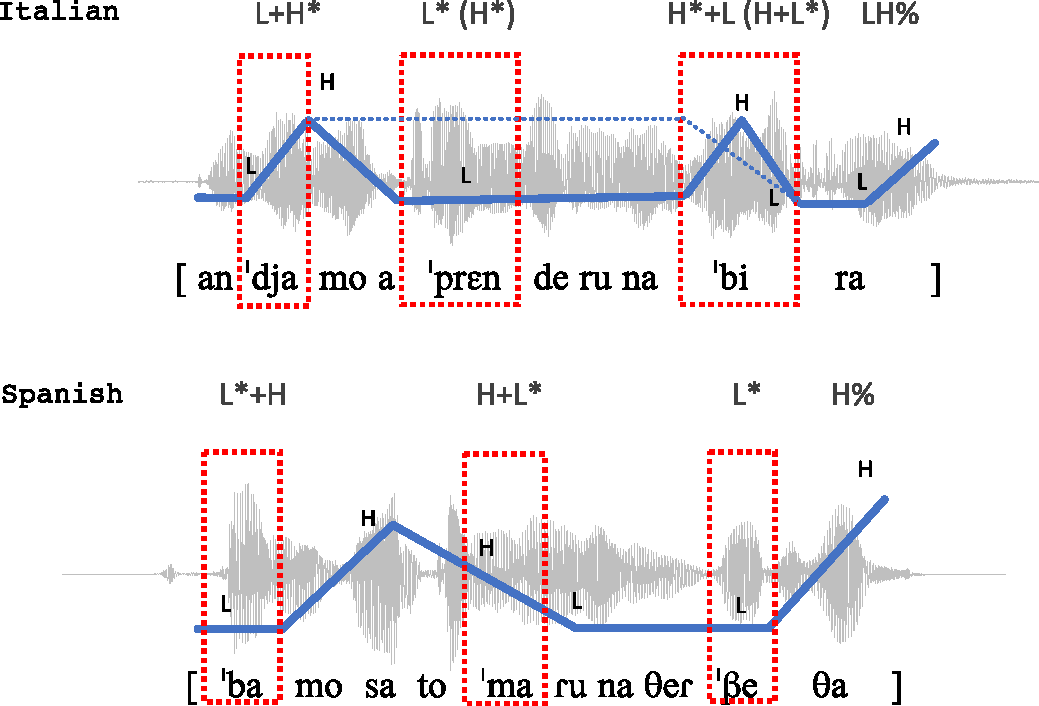
\includegraphics[width=.8\textwidth]{figures/a05HabilDiscussion-img012.pdf}



\caption{Idealized contours of neutral yes/no questions in L1 Italian and L1 Spanish.}
\label{fig:5.8}
\end{figure}

\begin{figure}

%%\includegraphics[width=\textwidth]{figures/a05HabilDiscussion-img013.emf}
\begin{tikzpicture}
\tikzset{every node/.style={font=\small}}
\begin{axis}[
  ybar=4pt,
  axis lines*=left,
  width = \textwidth,
  height=.3\textheight,
  ymin = 0,
  ymax = 100,
  ylabel = Accuracy \%,
  xtick = {1,2,3,4},
  xticklabels = {PAI,
  PAM,
  NA,
  BT,
  },
%  enlarge x limits = .06,
  bar width = 10,
  x tick label style = {font=\small},
  nodes near coords,
  legend pos = north west,
  legend columns = -1,
]
\addplot+[color = black, opacity = .2]
coordinates{
(1,60)
(2,45)
(3,70)
(4,92)
};
\addplot+[color = black, opacity = .5]
coordinates{
(1,40)
(2,45)
(3,57)
(4,75)
};
\addplot+[color = black, opacity = 1]
coordinates{
(1,32)
(2,67)
(3,52)
(4,27)
};
\legend{``German'' Spanish,``Czech'' Spanish,``Czech'' Italian}
\end{axis}
\end{tikzpicture}



\caption{Accuracy in neutral yes/no questions broken down by tonal event and learner variety. ``Ideal L1 speaker'': Spanish: L*+H (H+L*) L* H\%; Italian: L+H* (H*/L*), H+L*/H*+L LH\%.}
\label{fig:5.9}
\end{figure}


In short wh-questions (\textit{What time is it? What is your name?}), the results revealed that the Czech L2 Spanish learners performed very well in producing nuclear accents in comparison with the L2 Italian learners, whose accuracy was lower. The interlanguage varieties did not differ substantially in the initial position. As for boundary tones, learners of Spanish showed the highest accuracy by ending wh-questions with either a L\% or a H\% boundary tone. However, Czech learners clearly realized more L\% tones (52.5\%) in comparison to German learners (32.5\%) in those two wh-questions. Interestingly, Czech learners of Italian tended to realize wh-questions with different types of a high tone (H\%, LH\%, !H\% and H!H\%), similarly to what they did in L2 Italian yes/no questions. L2 Italian showed very low accuracy in nuclear position, since the learners used more L* patterns. With regard to longer and non-neutral wh-questions, the L1-L2 transfer was even more obvious. I assume that the length of the utterance and additional pragmatic meanings make acquisition more difficult (see also \citealt{JunOh2000}).


\begin{figure}

%%\includegraphics[width=\textwidth]{figures/a05HabilDiscussion-img014.emf}
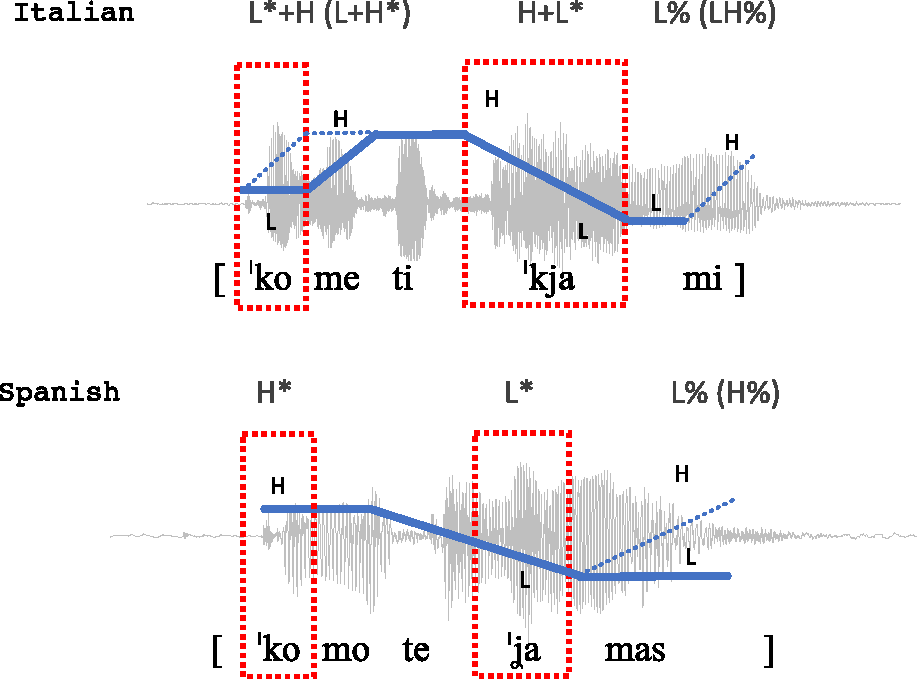
\includegraphics[width=.8\textwidth]{figures/a05HabilDiscussion-img014.pdf}



\caption{Idealized contours of neutral wh-questions in L1 Italian and L1 Spanish.}
\label{fig:5.10}
\end{figure}

\begin{figure}

%%\includegraphics[width=\textwidth]{figures/a05HabilDiscussion-img015.emf}

\begin{tikzpicture}
\tikzset{every node/.style={font=\small}}
\begin{axis}[
  ybar=4pt,
  axis lines*=left,
  width = \textwidth,
  height=.3\textheight,
  ymin = 0,
  ymax = 100,
  ylabel = Accuracy \%,
  xtick = {1,2,3},
  xticklabels = {PAI,
  NA,
  BT,
  },
%  enlarge x limits = .06,
  bar width = 10,
  x tick label style = {font=\small},
  nodes near coords,
  legend pos = north west,
%  legend columns = -1,
]
\addplot+[color = black, opacity = .2]
coordinates{
(1,33)
(2,66)
(3,95)
};
\addplot+[color = black, opacity = .5]
coordinates{
(1,36)
(2,83)
(3,93)
};
\addplot+[color = black, opacity = 1]
coordinates{
(1,40)
(2,12)
(3,40)
};
\legend{``German'' Spanish,``Czech'' Spanish,``Czech'' Italian}
\end{axis}
\end{tikzpicture}



\caption{Accuracy in neutral wh-questions broken down by tonal event and learner variety. ``Ideal L1 speaker'': Spanish: H* L* L\%/H\%; Italian: L*+H/L+H* H+L*, LH\%/L\%.}
\label{fig:5.11}
\end{figure}


Finally, the vocatives (initial calls) showed that German learners performed much better than Czech learners in Spanish, with Italian learners having the most difficulties with the target patterns in that they realized falling instead of rising nuclear accents (\figref{fig:5.12}). One of the explanations was that the tone H*+L is overgeneralized in this position, just as in the other type of sentences we saw above, and that learners might be using the tone as a typical “Italianish” feature. I will come back to this issue later.


\begin{figure}

%%\includegraphics[width=\textwidth]{figures/a05HabilDiscussion-img016.emf}
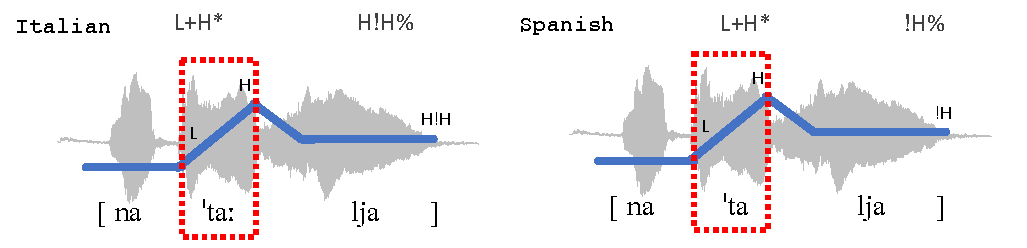
\includegraphics[width=\textwidth]{figures/fig512.pdf}
\caption{Idealized contours of vocatives in L1 Italian and L1 Spanish.}
\label{fig:5.12}
\end{figure}

\begin{figure}

%%\includegraphics[width=\textwidth]{figures/a05HabilDiscussion-img017.emf}
\begin{tikzpicture}
\tikzset{every node/.style={font=\small}}
\begin{axis}[
  ybar=4pt,
  axis lines*=left,
  width = .6\textwidth,
  height=.3\textheight,
  ymin = 0,
  ymax = 100,
  ylabel = Accuracy \%,
  xtick = {1,2},
  xticklabels = {
  NA,
  BT,
  },
  enlarge x limits = .5,
  bar width = 10,
  x tick label style = {font=\small},
  nodes near coords,
  legend pos = outer north east,
%  legend columns = -1,
]
\addplot+[color = black, opacity = .2]
coordinates{
(1,100)
(2,75)
};
\addplot+[color = black, opacity = .5]
coordinates{
(1,85)
(2,30)
};
\addplot+[color = black, opacity = 1]
coordinates{
(1,30)
(2,35)
};
\legend{``German'' Spanish,``Czech'' Spanish,``Czech'' Italian}
\end{axis}
\end{tikzpicture}



\caption{Accuracy in vocatives broken down by tonal event and learner variety. ``Ideal L1 speaker'': Spanish: L+H* !H\%; Italian: L+H* H!H\%.}
\label{fig:5.13}
\end{figure}


To conclude, differently strong deviations were observed in all three L2 varieties. These deviations include either “completely” non-target-like productions (e.g., the use of L\% instead of H\%) or “slightly” diverging productions (e.g., the use of H\% instead of LH\%, L+H* instead of L+<H*, etc.). In all cases, the role of L1 was quite crucial, in a positive as well as a negative way. I will discuss the findings within the LILt below (\sectref{sec:5.3}). If we calculate the average accuracy for the three interlanguages, we see that German learners of Spanish show a 62.8\% accuracy rate, Czech learners of Spanish 58.8\% and Czech learners of Italian 49.6\%. The fact that Czech learners performed worse in L2 Italian can be associated with the larger number of differences between L1 Czech and L1 Italian. Summing up, German learners’ overall performance in L2 Spanish was better in terms of intonation, which can be linked to more positive transfer. However, German learners performed slightly worse at the segmental level. This raises a question as to which of the learner groups exhibit a stronger foreign accent: the group with less accurate suprasegmentals or the group with less accurate segments? My students ran a pilot experiment on foreign accent rating with five native raters (speakers of Peninsular Spanish) and found out that German learners were evaluated with a stronger accent than Czech learners, independently of the type of sentence.\footnote{In this experiment, 10 advanced German and 10 advanced Czech learners were rated. The evaluated material comprised five sentences per speaker (\textit{Marisa come mandarinas,} \textit{¿Tienen mandarinas?}, \textit{¡Es John Travolta!}, \textit{¿Qué hora es?} and \textit{¡Natalia!}) that were repeated twice in the experiment. In addition, 70 fillers (recordings of L1 Spanish and other L2 learners from five different L1 backgrounds) were included in the experiment and the sentences were randomized. I would like to thank my Master’s students Hanne Ladewig, Nils Puchert, Luisa Sprehe, Anna Tillner Stortini and Maximilian Wilde for their work and effort in this seminar project.} This preliminary (but statistically significant) result suggests that the L1 background contributes to the overall perceived degree of foreign accent and that segmental deviances have a greater impact on accentedness than intonation. It cannot be ruled out that the contribution of intonation in foreign accent would change with other language combinations (for example, L1 Italian “sing-song” intonation in L2 Spanish).


\subsection{Didactic implications}\label{sec:5.2.2}

Based on the accuracy findings reported in the previous section we might ask whether and how intonation can be improved in an L2. First of all, we should underline that the results for accuracy revealed quite a positive picture if we think that the learners had never been trained for intonation at all and that their knowledge was purely implicit or intuitive (in  \citegen{Kivistö-deSouza2015} sense). Of course, all the learners had been exposed to native speakers and received different amounts of “native” input (\sectref{sec:3.3}). I believe that further improvement in L2 intonation could be achieved by an increase in learners’ phonological awareness. Specific intonation training, including imitation tasks and techniques involving the visualization of pitch has yielded positive results in previous studies (see, e.g., \citealt{Chun1998, NiebuhrEtAl2017}, \sectref{sec:1.4.2} and \sectref{sec:2.1.4} for further references). To the best of my knowledge, no material of this kind for Czech and German learners of L2 Spanish and L2 Italian has been proposed to date (but see  \citealt{CortésMoreno2002, Elvira-García2016} for Spanish intonation training and \citealt{Mocciaro2014} and \citealt{Nicora2020} for Italian intonation training) and this calls for development of teaching and learning strategies to improve students’ L2 pronunciation in terms of intonation. In order to improve learners’ production, it is crucial to make transmission of L2 intonation in classes and teaching material as transparent, practical and simple as possible so it can be used by instructors who are not familiar with intonation research.


In \sectref{sec:2.1.2}, we became familiar with the \citegen{CEFR2018} latest proposal, which includes several prosodic features but lacks a more tangible description. \tabref{tab:5.1} offers a preliminary proposal -- which should be developed and tested further -- for how intonation skills could be integrated into the \textit{Phonology control} rubric in CEFR. Although there is no “standard” intonation for these languages, it is recommended that learners orientate themselves towards the L2 variety they are exposed to. It goes without saying that there must be professional instruction in classes so that learners are able to achieve such competences.

\begin{table}
\begin{tabularx}{\textwidth}{X}
		\lsptoprule
		\multicolumn{1}{l}{{Basic users (A1--A2)}}\\\midrule
		 Can perceive as well as produce the variable stress placement in isolated words.
		 
		 Can produce prenuclear as well as nuclear pitch accents in simple declarative sentences.
		 
		 Can produce typical contours of short neutral declaratives, neutral yes/no questions as well as neutral wh-questions.\\
		\midrule
		\multicolumn{1}{l}{{Independent users (B1--B2)}}\\\midrule
		Can produce intonation patterns of exclamatives, vocatives, imperatives.
		
		Can produce boundary tones in longer and syntactically more complex sentences.
		
		Can produce prosodic focus marking.\\ 
		\midrule
		\multicolumn{1}{l}{{Proficient users (C1--C2)}}\\\midrule
		Can understand and produce contours of different sentence types with additional meanings (certainty, incredulity, irony etc.).
		
		Can also use specific expressions (discourse elements or interjections) which may interact with prosody.\\
		\lspbottomrule
	\end{tabularx}
\caption{\label{tab:5.1}Proposed intonation skills for Spanish and Italian as L2s that could be integrated into a CEFR rubric.}
\end{table}

\section{Discussion of the results within the L2 Intonation Learning theory}\label{sec:5.3} %5.3 /

The main assumption underlying the LILt is that intonation deviations and CLI occur in four different dimensions. This is fully supported by the results of the present study.

\subsection{L2 patterns in the systemic dimension}\label{sec:5.3.1}

We started out with the following two research questions: \textit{Did L2 learners omit pitch accents and boundary tones that do not form part of their native language inventory? Did they transfer native patterns that are not present in the target language?}


In order to be able to answer the first question, I will briefly review the Spanish and Italian patterns which are not present in L1 Czech and L1 German (see \chapref{ch:2}, \sectref{sec:2.3.2.4}, \tabref{tab:2.8a}). Spanish exhibits three tonal patterns that are not included in the German and Czech intonational inventories: L+<H*, LHL\%, L!H\%. The first one is a rising tone in the tonic syllable with a late peak in the posttonic syllable (L+<H*), representing the typical prenuclear pitch accent of statements in most Spanish dialects. German learners showed particular difficulties with this tone in initial prenuclear positions and managed to realize it in only 17.5\% of all cases. Instead, they produced L*+H in more than half of the cases (the difference between L*+H and L+<H* consists in the shape of the rise in the tonic syllable). Czech learners, in contrast, had less difficulty producing this pattern, using it in 45\% of all cases. This is due to a phonetic coincidence: in Czech, an accentual phrase /L* Ha/ in statements corresponds phonetically to L+<H* in Spanish.\footnote{This holds at least for the three-syllable paroxytone words which were used in the data of the present study. Future research should include words with a different syllable length and stress position in order to test whether the phonetic implementation of the tonal events will cause more difficulties for learners.}  It must be added that in medial positions of statements, Czech learners of Spanish used L+<H* in 10\% of cases, whereas German learners did not produce this tone at all. In \sectref{sec:5.1} I speculated that this might be due to negative transfer and a lesser degree of importance of this position for meaning. Another Spanish pattern reported in the literature that does not exist in Czech or German is a tritonal LHL\% boundary tone, consisting of a rise-fall F0 movement (see, e.g., \citealt{AguilarEtAl2009}). This boundary tone is described for exhortative requests in Spanish. The present study does not include requests in the final analysis (see \chapref{ch:3}), but during the recordings I noticed that the learners were unaware of this tonal pattern in this type of sentence, just as they were unaware of L!H\% in statements of the obvious (recall that only two out of a total of 40 learners used the L!H\% correctly). It should be added that Czech and German yes/no questions include LH\%, which is phonetically close to the L!H\%.



With regard to L1 Italian, L*+>H (or H+L*+H in my annotation), H*+L with its variant L+H*+L and L!H\% are not present in L1 Czech. The L*+>H pattern, characterized by a F0 fall followed by a rise to an early peak in the tonic syllable, has been attested for exclamatives in relatively few Italian dialects (Turin, Milan, Rome, Lecce and Lucca) (see \citealt{GiliFivelaEtAl2015}). Its low frequency and semantic limitation might explain why it was not very common in learners’ productions: L*+>H appeared merely three times in nuclear positions (in two biased yes/no questions and one statement of the obvious), probably as a phonetic variant or mixed form of other structural element. As for H*+L (L+H*+L), characteristic of nuclear accents of contrastive focus and emphasis in many Italian dialects, all learners acquired and produced this pattern to varying degrees, some learners used it more frequently than others (see \citealt{Pešková2022b} for details). I tried to interpret this individual variation in terms of the proficiency level of the learners and found the following tendency: intermediate learners (level B) realized this tone in 75 cases, while advanced learners (level C) did so in 62 cases. Moreover, less proficient learners realized this tone more often even in prenuclear positions (10 cases vs. 4 cases). This finding nicely demonstrates that the occurrence of the “overgeneralized” pattern diminishes as learners reach a higher proficiency level (see \sectref{sec:5.4} for a further discussion of the overall developmental sequences). As I suggested above (see \sectref{sec:5.1} and \sectref{sec:5.2.1}), the “overuse” of this pattern could be related to prosodic overgeneralization. I also suppose that learners overgeneralize precisely this tone because it is used very frequently in spoken Italian and is perceptually very prominent in comparison to other types of tones.



Finally, the L!H\% boundary tone is described in counter-expectational yes/no questions in Lecce Italian. In the present data, the learners realized this tone in a total of ten biased yes/no and wh-questions. As mentioned above, its use could be seen as a phonetic variation of LH\%, typical of interrogatives in L1 Czech and the majority of Italian dialects. In other words, the problem may be related to the phonetic rather than the systemic dimension (see \sectref{sec:5.3.2}).



As for the second question, the answer is yes: learners do transfer L1 patterns that are not present in the target language. For example, some German learners of Spanish transferred their L1 H-\^{}H\% boundary tone (a high plateau with an upstepped final rise on the last syllable) to neutral yes/no questions in their L2 Spanish. By the same token, many Czech learners, especially female participants, used Lː\% in familiar insistent requests in their L2 Italian and their L2 Spanish.\footnote{I assume that the final lengthening (Lː\%) is phonological in Czech because it conveys a different meaning when compared with L\% \citep{PeškováForthcoming}.} Although requests were not analysed systematically, I observed the lengthening in this type of sentence in the course of the recordings. Additionally, L1 influence was attested in L2 biased wh-questions produced by Czech learners, who tended to add pauses between the wh-word and the rest of the question (see \citealt{Pešková2021}).



We can summarize the main findings in this dimension as follows. First, L2 learners omit only some of the pitch accents and boundary tones that do not form part of their native language inventory. Their omission and the expression of new patterns can be connected with their frequencies and the contexts in which they are used; phonetic similarities between the target language and the L1 also play a role. Second, L2 learners also transfer their L1 patterns that are not present in the target language. However, we saw that these patterns are often phonetically similar to the TL and do not affect any changes in semantic meaning. Hence, many intonational deviations and transferred phenomena in the systemic dimension may be closely related to other dimensions. I will summarize the tonal inventories of the L2 varieties in \sectref{sec:5.3.4}, when discussing the \textit{frequency} dimension.


\subsection{L2 patterns in the phonetic dimension}\label{sec:5.3.2}

Here two questions were formulated: \textit{Did learners have particular problems with the phonetic realization of target contours? Did learners have more difficulties in acquiring new patterns or phonetically different categories?}


Though the present study did not analyse the data in fine phonetic detail, the findings suggest that learners have particular difficulties with prosodic parameters such as alignment, range, slope and duration and probably intensity too. In the previous section, we saw that learners had problems with L+<H* and L!H\% that might be connected with alignment and pitch range difficulties. Additionally, German learners exhibited an earlier slope and peak in the realization of L*+H tones when compared with Czech learners and Spanish natives. Moreover, Czech learners showed mixed shapes of high boundary tones (H\%, !H\%, H!H\%) in L2 Italian and L2 Spanish questions that were very similar to those attested in L1 Czech (see \citealt{PeškováEtAl2018}). In L2 Spanish yes/no questions, Czech learners also had problems with accurate pitch changes in initial prenuclear positions showing reduced pitch excursions which could be due to CLI. As for duration parameters, we observed, for instance, a case of “overexaggerated” length of stressed syllables in L2 Italian vocatives.



Broadly speaking, the observed tendencies support Flege’s \textit{Speech Learning Model} (SLM) assumption that L2 sounds that are phonetically similar to those sounds of L1 are more difficult to acquire than “new” L2 sounds (this view is also supported by \citealt{Zárate-Sández2015} who examined the perception and production of intonation by English-native speakers of Spanish). In the data, Czech learners had less trouble learning the Italian (L+)H*+L target pattern in a nuclear position than German learners the rising tone (L+<H*) in a prenuclear position. Of course, this preliminary generalization needs to be taken with caution because the present study did not compare the phonetic details of (L)+H*+L tones in L2 with L1 Italian and we cannot support the Flege’s model with perception data.



All in all, divergences in form may cause many troubles in L2 intonation, similarly to what we saw in the case of segments in target language. Nevertheless, a different form of the tonal event does not represent the only difficulty.


\subsection{L2 patterns in the semantic dimension}\label{sec:5.3.3}

In the semantic dimension functions and meanings of utterances are closely linked. The related research question was: \textit{Did learners use intonation to signal functions in a TL-appropriate way or did they instead transfer patterns from their L1?}


The overall findings of the present study reveal that learners were able to distinguish and reproduce the semantic meanings of sentences (e.g., statements vs. questions, exclamatives vs. imperatives, etc.) but had more difficulties acquiring the pragmatic meaning of utterances (e.g., neutral vs. biased). In the marked contexts, in which additional pragmatic nuances and emotions were involved, the learners either realized neutral patterns and/or mostly transferred patterns from their L1. For example, many learners produced counterexpectational echo yes/no questions and wh-questions with a typical neutral rise. This indicates that learners simplify forms probably due to their low pragmatic awareness in the L2. It is not excluded that intimidating effects of recording settings also play a role.



We saw the difficulties related to the realization of target patterns in this dimension throughout \chapref{ch:4}. To give some examples, German learners of Spanish produced L*+H in prenuclear positions in statements. However, this pitch accent represents prenuclear pitch accents of Spanish yes/no questions. So, theoretically, Spanish natives would interpret the L2 prenuclear material as a question and not as a statement. In L2 neutral vocatives, the Czech learners tended to produce L\%, which is characteristic of declaratives or wh-questions, instead of the target (H)!H\% patterns. In statements of the obvious, both Czech and German learners used mostly L1-based focus patterns (L+H* L\%) instead of the target L+H* L!H\% contour.



Furthermore, the results indicate that learners have problems not only with the functions of the target patterns but also with the position of the tonal events (we could call this the \textit{syntactic dimension}). Learners show also more difficulties and transfer phenomena when the sentences are longer. For example, in statements, learners have more trouble with medial positions, and in longer or pragmatically marked questions they struggle with the correct placement of prominence (see also \citealt{JunOh2000} for similar findings in L2 Korean questions produced by American English speakers).



It should be noted that I did not report differences concerning combinations of nuclear accents with boundary tones, that is, nuclear configurations, where languages may differ substantially too (see an overview in \chapref{ch:2}, \sectref{sec:2.3.2.4}, \tabref{tab:2.8a}). I made this decision for two reasons. First, the results yield such a high number of combinations that the data appear to be far too complex for interpretation. Second, although nuclear configurations \textit{per se} have the strongest impact for meaning, the rest of the F0 contour is also responsible for how a sentence sounds. The present study demonstrates in many cases that transfer concerns not only categories (pitch accents, boundary tones) but the entire pitch track of a sentence. L1 transfer of such melodic constructs is apparent especially in wh-questions, in which the traditional ToBI labelling system and the treatment of categories according to stressed syllables show limitations (see, e.g., \citealt{Kimura2006}, who points out mismatch of stress and accent in Spanish within the ToBI framework). The findings also suggest that L2 learners store and memorize the whole contours or phases of these contours rather than tonal events (pitch accents, boundary tones) separately (see \citealt{TorreiraGrice2018} and \citealt{Pešková2021} for further discussion). I therefore believe that intonation contours must be dealt with in a more holistic way in future.


\subsection{L2 patterns in the frequency dimension}\label{sec:5.3.4}

The aim of this dimension is to compare whether the same category is used more or less frequently in one language than in the other. The question concerning this dimension was: \textit{Did learners prefer certain patterns more often, and if so, why?}


Even when languages share the same patterns, they may differ in the frequency and distribution of tonal events. For example, the complex boundary tones L!H\%, !H\% and LHL\% are less frequent than L\% and H\% in L1 Spanish. The same applies to L*+>H, H!H\% and L!H\% in L1 Italian. However, I feel that precise information on frequencies of intonation primitives for each language (and for each speaker) is lacking. This dimension also creates the dilemma of how to choose suitable methods and material for determining and comparing such frequencies. Since the interpretation of this dimension is a little bit difficult, I will focus only on differences (in frequency) between the interlanguages. As we will see, these can be attributed to an influence of the L1, on the one hand, and the type of target language, on the other.



With regard to boundary tones (at the BI 4 level) (\tabref{tab:5.2}), German learners of Spanish produce H\% at the highest rate (46.6\%), whereas Czech learners of Italian and Spanish realize L\% most frequently (45.9\% and 49.5\%, respectively). This is related to the frequencies of these tones in L1 questions. The reason behind the higher frequency of !H\% in “Czech” Italian than in “Czech” Spanish might be due to the L1 variety of learners: learners of L2 Italian came predominately from Moravia, where !H\% is more common BT of yes/no questions than in Bohemian varieties \citep{PeškováEtAl2018}. Another explanation could be that !H\% is a result of a less successful phonetic implementation of the target pattern /LH\%/ in Italian questions.



No particular differences were found in the realization of boundary tones at the intermediate phrase. In contrast, the interlanguages differ substantially in the frequency of high boundary tones (Hi) at the very beginning of sentences: whereas only four cases were detected in “German” L2 Spanish, 35 and 15 cases were found in “Czech” L2 Spanish and L2 Italian.


\begin{table}
\begin{tabularx}{\textwidth}{QlYYY}
\lsptoprule
{Tonal event} & {ToBI} & {“German” Sp.} & {“Czech” Sp.} & {“Czech” It.}\\
\midrule
\multirow[t]{8}{=}{Boundary tones at IP} & L\% & 41.8 & {\bfseries 49.5} & {\bfseries 45.9}\\
& H\% & {\bfseries 46.6} & 35.3 & 25.5\\
& !H\% & 6.1 & 5.2 & 14.7\\
& H!H\% & 0.5 & 2.6 & 0.5\\
& HL\% & 2.4 & 4.7 & 2.1\\
& LH\% & 2.4 & 2.4 & 8.8\\
& L!H\% & 0.3 & 0.3 & 2.6\\
\midrule
& {\itshape N} & {\itshape 380} & {\itshape 382} & {\itshape 388}\\
\midrule
\multirow[t]{4}{=}{{Boundary tones at ip}} & L- & {\bfseries 86.0} & {\bfseries 78.0} & {\bfseries 77.8}\\
& L(!)H- & 2.3 & 2.4 & 3.7\\
& (!)H- & 11.6 & 19.5 & 18.5\\
\midrule
& {\itshape N} & {\itshape 43} & {\itshape 41} & {\itshape 54}\\
\lspbottomrule
\end{tabularx}

\caption{\label{tab:5.2}Frequencies of all realized boundary tones according to the interlanguage.}
\end{table}


Furthermore, several important differences in pitch accents were manifested (\tabref{tab:5.3}). First, the CLI can explain the differences between Czech and German learners of Spanish observed in the rates of prenuclear pitch accents. In initial prenuclear positions, L*+H clearly predominates in German learners of Spanish, whereas Czech learners show larger variation that could be due to the fact that Czech is a phrase language, in which the accentual phrases show more F0 variability or flexibility. In addition, Czech learners produced a higher number of H+L* in initial or final positions, in contrast to German learners. In medial positions of all sentence types, we see the following frequency patterns: H+L* in “German” Spanish (35.8\%), H* in “Czech” Spanish (35\%) and L* in “Czech” Italian (37.1\%). In nuclear positions, L+H* is the predominant pattern in both “German” (57.1\%) and “Czech” Spanish (43.3\%), whereas H+L* (25.8\%) followed by L* (21.9\%) dominates in “Czech” Italian.


\begin{sidewaystable}
\begin{tabularx}{\textwidth}{lYYYYYYYYY}

\lsptoprule

{ToBI} & \multicolumn{3}{c}{{Initial prenuclear}

{pitch accents}} & \multicolumn{3}{c}{{Medial prenuclear}

{pitch accents}} & \multicolumn{3}{c}{{Nuclear accents}}\\
\cmidrule(lr){2-4}\cmidrule(lr){5-7}\cmidrule(lr){8-10}
& ``German''

 Spanish & ``Czech''

 Spanish & ``Czech''

 Italian & ``German''

 Spanish & ``Czech''

 Spanish & ``Czech''

 Italian & ``German''

 Spanish & ``Czech''

 Spanish & ``Czech''

 Italian\\
 \midrule
{H*} & 14.9 & 19.5 & 20.2 & 26.7 & {\bfseries 35.0} & 19.4 & 1.9 & 3.3 & 4.8\\
{L*} & 7.8 & 7.4 & 13.1 & 5.8 & 21.7 & {\bfseries 37.1} & 29.5 & 31.4 & 21.9\\
{L*+H} & {\bfseries 44.3} & {\bfseries 29.1} & {\bfseries 30.9} & 8.3 & 3.3 & 7.0 & 3.8 & 1.2 & 7.8\\
{L+<H*} & 16.3 & 20.6 & 6.0 & 3.3 & 7.5 & 1.1 &  &  & \\
{L+H*} & 11.7 & 10.6 & 19.9 & 20.0 & 9.2 & 9.7 & {\bfseries 57.1} & {\bfseries 43.3} & 11.6\\
{H+L*} & 5.0 & 12.8 & 8.2 & {\bfseries 35.8} & 23.3 & 21.0 & 7.6 & 18.1 & {\bfseries 25.8}\\
{H*+L} &  &  & 0.7 &  &  & 2.7 &  & 2.1 & 15.1\\
{L+H*+L} &  &  & 1.1 &  &  & 2.2 &  & 0.5 & 12.3\\
{(H)+L*+H} &  &  &  &  &  & 0.0 &  & 0.0 & 0.7\\
\midrule
{\itshape N} & {\itshape 282} & {\itshape 282} & {\itshape 282} & {\itshape 120} & {\itshape 120} & {\itshape 186} & {\itshape 420} & {\itshape 420} & {\itshape 438}\\
\lspbottomrule
\end{tabularx}

\caption{\label{tab:5.3}Frequencies of all realized pitch accents according to the interlanguage (the most frequent patterns are marked in bold).}
\end{sidewaystable}


At the end of this section, it should be mentioned that the LITt does not account for the syntactic and stylistic dimensions. Syntax phenomena and especially word order must be another prerequisite of successful intonation learning. I cannot provide evidence from the intonation questionnaire analysed here, but I noticed certain (morpho-)syntactic deviations (non-native word order, overuse of pronominal subjects) during the free interviews, especially in some of the productions uttered by intermediate learners. As for stylistics, \citet{Ulbrich2008} (cited also in \citealt{Mennen2015}) found that German learners of Belfast English (BfE) found it difficult to acquire stylistic variation, notably in speaking style and register. She concluded that the learners were not able to vary prosodic features appropriately in accordance with the degree of formality or speaking style (or were not aware of them), whereas native speakers of BfE tended to change their regional markers depending on whether they were producing read, semi-spontaneous or spontaneous speech. Moreover, we should cover the interplay of intonation with other prosodic and segmental phenomena (and even paralinguistic features), and include the role of universal constraints such as markedness in the acquisition of L2 intonation. For example, final rises can be considered more marked for statements than falls, at least in Indo-European languages. The markedness issue begs the question of whether learners prefer to produce unmarked patterns to marked ones. This is indeed a difficult issue, since linguists have not reached agreement on which intonation patterns are marked and which are not. However, the present study shows that the learners tend to overuse rising patterns in yes/no and wh-questions, even when L1 transfer implies falling patterns. Interestingly, the same tendency was reported in the study by \citet{SantiagoDelais-Roussarie2015b, SantiagoDelais-Roussarie2015a} on L2 intonation in French produced by Mexican Spanish learners. As speculated in \sectref{sec:5.3.3}, this behaviour might mean either an acquisition strategy (simplification of forms) or an overgeneralization of an unmarked, “universal” form, if we consider the rise a typical feature of questions (see, e.g., \citealt{Bolinger1972b, Cruttenden1997}).



Concluding, we can confirm the LILt’s hypothesis “that not all intonation dimensions constitute the same amount of difficulty in L2 learning.” Moreover, not all intonation dimensions constitute the same amount of difficulty for every learner. Not surprisingly, the data exhibited strong inter-learner variation. The present study has focused so far on the role of the L1 and cross-linguistic influence in order to explain variation observed in L2 intonation. In 5.4. I will discuss the important research question of whether the obtained proficiency level would help to explain variation further and whether any developmental sequences in terms of L2 learning could be determined.


\section{Variation and developmental sequences}\label{sec:5.4} %5.4 /

Since the present study is not longitudinal, differences between intermediate and advanced learners (\textit{Proficiency level}) were assumed to give us an answer on intonational development. The previous research on the perceptual and productive accuracy of segments provides enough evidence of the developmental sequences and improvement toward target-like pronunciation at higher proficiency levels (see, e.g., \citealt{Hansen2004} for the acquisition of codas in L2 English with L1 Vietnamese; \citealt{Stella2012} for the alignment of pitch accents in L2 German with L1 Italian; \citealt{PeškováEtAl2017} for the acquisition of the vowel quantity in L2 Spanish with L1 Czech). During the recordings I noticed that learners of C levels had more fluent speech (showing less dysfluencies such as pauses and other interruptions) and mastered various grammatical aspects very successful. Hence, there was no particular reason to believe intonation would be different (see, e.g., \citealt{Trimble2013} and \citealt{Zárate-Sández2015} for the acquisition of tonal patterns in L2 Spanish by L1 English natives).


The data, however, do not afford us any satisfying answer as the effect of the \textit{Proficiency} factor comes out statistically insignificant: whereas \textit{L1 language} reveals significant differences between German and Czech learners of Spanish ($\chi^2(12) = 71.06,\allowbreak p = 0.000$), \textit{Proficiency level} shows no significance ($\chi^2(12) = 19.524,\allowbreak p = 0.077$). L2 Italian compared with L2 Spanish produced by Czech learners shows a similar tendency, namely, statistically high significant differences for \textit{Target language} ($\chi^2(13) = 211.66,\allowbreak p = 0.000$) but no significance for \textit{Proficiency level} (B vs. C) ($\chi^2(13) = 11.63,\allowbreak p = 0.559$). I will attempt to interpret what might be behind this unexpected finding.



An explanation for the lack of clearer differences between B and C levels in the present study might be that the majority of the learners were proficient B2 and C1 learners and that these two groups are very close to each other. However, this interpretation leaves at least one doubt. In \citet{PeškováEtAl2017} we showed that Czech advanced learners of L2 Spanish (C) were more accurate in producing the length of the accented vowels in comparison to intermediate learners (B), and the finding was statistically significant. The important point here is that the data came from the same individuals. In \citet{PeškováEtAl2017} we analysed only the data from a word-list reading task (see \chapref{ch:3}). Indeed, it is not excluded that the degree of CLI and accuracy may depend on the particular task used (see, e.g., \citealt{ColantoniEtAl2016b}).



An alternative assumption here is that L2 intonation is acquired early in the acquisition process -- at B2 level at the latest -- and becomes fossilized at that point (or even earlier). \citet{Sims1989} claims that fossilization is closely related to simplifying learning strategies, which are common to all learners. Many L2 learners that I interviewed self-reported that understanding and being understood was the most important goal in their L2 acquisition, taking priority over correct grammar or native-like pronunciation. In other words, communicative function took precedence for them over linguistic form. This “simplifying learning strategy” can be one of the crucial factors for understanding why the learner’s \textit{interlanguage} will cease to develop in certain domains (see also \citealt{Corder1967, Selinker1993}). Intonation is probably affected more strongly by fossilization than other phenomena. Of course, the point at which fossilization occurs can vary from individual to individual and depend on a large number of factors. In \sectref{sec:2.1} we discussed several aspects that are supposed to play a role in L2 speech and determine a degree of foreign accent. In general, there can be a relation to the age of learning (AOL), the length of experience or residence (LOR) in a target-language-speaking country and the related quality and quantity of input as well as formal instruction and increasing phonological awareness. Previous studies on L2 Spanish intonation (e.g., \citealt{HenriksenEtAl2010, Trimble2013, Craft2015}) have reported a positive effect of a stay abroad programme in the intonational development and changes toward a more native-like pronunciation. In \citet{Pešková2022b}, however, I report that LOR, AOL and the amount of the active use of a L2 per week do not impact significantly the accuracy in L2 intonation of non-neutral statements. For example, one advanced student of Italian (C2, Cz\_F\_38) who had spent five years in Italy showed more intonation errors and had a stronger “Czech accent” in her L2 than one intermediate student who spent only five months abroad (B1, Cz\_F\_47). On the other hand, the former student was much more fluent in her spontaneous speech and very proficient in terms of grammar and vocabulary. Furthermore, intonation proficiency does not seem to go hand in hand with proficiency in other domains, segmental accuracy included. One German participant (B1, Ge\_F\_07) who had spent six months in Barcelona just before I recorded her for the experiment spoke with a typical Catalan “tune”, although her segmental performance included many L1-transferred features (aspirations, vowel reduction and mispronunciation of rhotics). With regard to LOR, there is another factor that may also play a role here. According to \citet{PiskeEtAl2001}, it is not only important how much time the learner spends abroad but also at what point in the acquisition process. The authors are of the opinion that the length of the experience is important especially when it takes place in the earlier phase of L2 learning in general. This means that learners should be exposed to a higher degree of input at the very beginning of their acquisition process. \citet[210]{PiskeEtAl2001} also claim that after L2 learners have spent a certain amount of time in a TL-speaking area, “increases in LOR will cease to have a further ameliorative effect on L2 pronunciation”. All of this -- in addition to aspects such as personal motivation and specific aptitudes -- may explain the individual differences and require further clarification in future.



All in all, the developmental sequences involved in the learning of L2 intonation leave open a number of questions for future research, in which longitudinal studies with individuals should play a central role. It must be emphasized that although no significant effect between the two levels was found, this does not mean that developmental sequences do not exist. If this were true, Czech learners of Italian would have shown the same L1-based patterns as Czech learners of Spanish, and the intonation accuracy would not have been so high. Prosodic overgeneralization -- here the overuse of H*+L in L2 Italian -- represents a clear piece of evidence for L2 interlanguage development.



The very last related question was whether we could predict which phenomena are more likely to become overgeneralized and fossilized. Functional constraints such as frequency effects, perceptual saliency, ease of articulation and perception have been said to be relevant for segments (\citealt[16]{ColantoniEtAl2015}). In terms of intonation, the findings of the present study and from the previous research (see \sectref{sec:1.4}., \sectref{sec:2.1}, \sectref{sec:2.4}) allow us to make the following predictions that will need further corroboration in future research (see \chapref{ch:6} for details):

\begin{description}
\item[\textit{Developmental L2 Intonation Hypothesis}:]
\begin{enumerate}[label=(\arabic*)]
\item[]
\item Phonological features of intonation are acquired earlier than phonetic features of intonation.
\item Pragmatically unmarked structures are acquired earlier than marked structures.
\item Patterns that exist in both L1 and L2 are acquired earlier than new patterns provided that they convey the same meaning.
\item Patterns with a strong semantic weight are acquired earlier than patterns with no changes in meaning.
\item Patterns that do not involve substantial changes in the semantic dimension fossilize faster.
\item Phonetically similar patterns that exist in both L1 and L2 fossilize faster than phonetically different patterns.
\item Patterns in functionally weaker positions fossilize faster than patterns in functionally stronger positions.
\item New but frequent and perceptually prominent patterns tend to be subject to overgeneralization.
\item Rising boundary tones (as unmarked or “universal” forms) tend to be overgeneralized in all types of questions.
\end{enumerate}
\end{description}

I would also suggest that these generalizations are characteristic of interlanguage intonation independently of learners’ L1 backgrounds. In addition, the results presented here reveal that the prosody of interlanguages in general is characterized by slower speech rate, dysfluencies, the omission of less frequent tonal patterns and the simplification of forms in pragmatically marked contexts.
